
\begin{figure}[H]
    \centering
    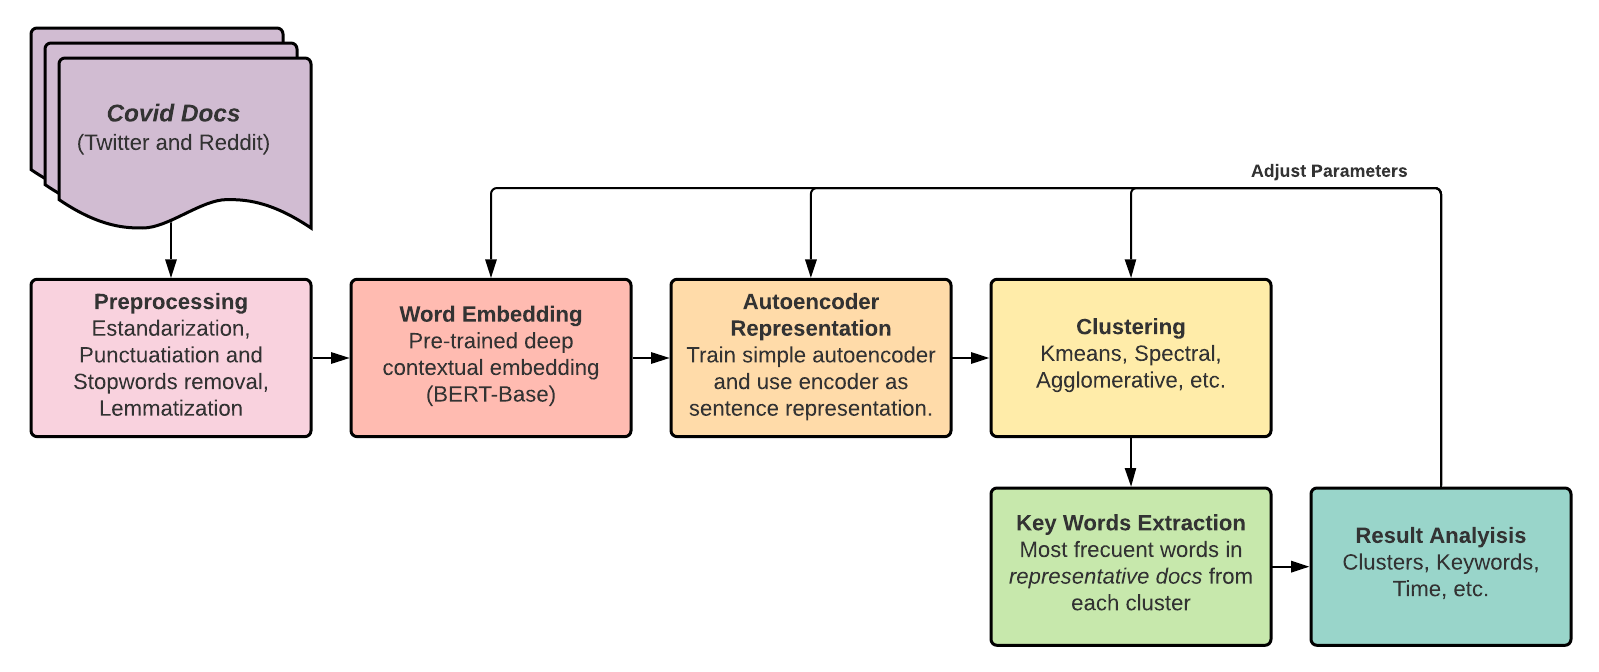
\includegraphics[width=\textwidth]{doc_hw04/images/TopicDetectionDiag.png}
    \caption{Metodología propuesta para la detección de tópicos utilizando \textit{deep sentence representation} y \textit{clustering}.}
    \label{fig:TopicDetectionDiag}
\end{figure}

El \textit{dataset} utilizado para detección de temas en tendencia corresponde documentos recogidos por los autores de dos fuentes diferentes \textit{Twitter} y \textit{Reddit} en inglés, español y francés. Por cuestión de tiempo de procesamiento se decidió excluir las noticias recopiladas. Si bien se tiene una gran cantidad de datos en inglés (más de 800.00 documentos) se decide utilizar únicamente alrededor de 135.000 datos con el fin de impedir que la cantidad de documentos favoreciera un idioma por encima de otro, y poder analizar con mayor imparcialidad. El total de documentos utilizados en cada caso se muestra en la tabla \ref{tab:docs}.
\subsection{Dataset}

\begin{table}[H]
\centering
\caption{Total de documentos utilizados por idioma}
\label{tab:docs}
\begin{tabular}{lrrrr}
\hline
\textbf{Idioma} & \textbf{Twitter} & \textbf{Reddit} & \textbf{Total} \\ \hline
Inglés          & 99.971           & 45.725          & 145.696        \\
Español         & 125.000          & 6.479           & 131.479        \\
Francés         &                  &                 &                \\ \hline
\end{tabular}
\end{table}

\subsection{Preprocesamiento}

El preprocesamiento de los datos se realizó siguiendo los siguientes pasos:
\begin{enumerate}
    \item Pasar todas las palabras a minúsculas.
    \item Eliminar signos de puntuación y caracteres especiales.
    \item Tokenizar las palabras.
    \item Lematizar las palabras.
\end{enumerate}

\begin{itemize}
    \item \textbf{Reddit original:}
    \begin{itemize}
        \item [\textbf{Inglés:}] Someone I am close to works in a factory called Dixon in Maryland. This person is one of only 2 people wearing a mask in the entire factory, including office staff. How this is acceptable I have no idea. The recklessness and denial in the face of a global pandemic is astounding. Companies not protecting employees in close proximity with masks wearing policy should be fined. It's criminal given what we know about transmission.
        \item [\textbf{Español:}] INER está al 100\% de capacidad por COVID y personal está agotado, advierte su director.
        \item [\textbf{Francés:}] Pourquoi autant mentir? On veut freiner et éliminer la contagion au Québec ou la nourrir comme on arrose un jardin? Je comprends pas.
    \end{itemize}
    \item \textbf{Reddit preprocesado:}
    \begin{itemize}
        \item [\textbf{Inglés:}] 'someone', 'close', 'works', 'factory', 'called', 'dixon', 'maryland', 'person', 'one', '2', 'people', 'wearing', 'mask', 'entire', 'factory', 'including', 'office', 'staff', 'acceptable', 'idea', 'recklessness', 'denial', 'face', 'global', 'pandemic', 'astounding', 'companies', 'protecting', 'employees', 'close', 'proximity', 'masks', 'wearing', 'policy', 'fined', 'criminal', 'given', 'know', 'transmission'
        \item [\textbf{Español:}]'iner', '100', 'capacidad', 'covid', 'personal', 'agotado', 'advierte', 'director'.
        \item [\textbf{Francés:}] 'pourquoi', 'autant', 'mentir', 'veut', 'freiner', 'éliminer', 'contagion', 'québec', 'nourrir', 'comme', 'arrose', 'jardin', 'comprends'
    \end{itemize}
    \item \textbf{Tweet original:}
    \begin{itemize}
        \item [\textbf{Inglés}] \#WorldBank “Living paper”: \#SocialProtection and Jobs - Responses to \#COVID19: A Real-Time Review of Country Measures; version 15 (May 14, 2021)
        \item [\textbf{Español:}] Madrid ha gastado ya, dicen aquí, 299 millones de euros en hacer frente a la pandemia... habiendo recibido 3.384 millones...
        \item [\textbf{Francés:}] La progression de la protection vaccinale contre la covid 19 permettra-t-elle prochainement d'assouplir les recommandations ? \#COVID19 \#VaccinationCovid 
    \end{itemize}
    \item \textbf{Tweet preprocesado:}\\ 
    \begin{itemize}
        \item [\textbf{Inglés:}] 'worldbank', 'living', 'paper', 'socialprotection', 'jobs', 'responses', 'covid19', 'realtime', 'review', 'country', 'measures', 'version', '15', 'may', '14', '2021'
        \item [\textbf{Español:}] 'madrid', 'gastado', 'dicen', 'aquí', '299', 'millones', 'euros', 'hacer', 'frente', 'pandemia', 'recibido', '3384', 'millones'
        \item [\textbf{Francés:}] 'progression', 'protection', 'vaccinale', 'contre', 'covid', '19', 'permettratelle', 'prochainement', 'dassouplir', 'recommandations', 'covid19', 'vaccinationcovid'
    \end{itemize}
\end{itemize}


\subsection{Extracción de características}
\subsection{\textit{Clustering}}
